\begin{problema}{Two Mysterious Alphabets from a Tree}{Standard}{Standard}{COJ}

Your task is to extract 2 alphabets from a binary tree which is composed of unsigned integers respecting the following rules. Let $n$ be the height of a tree. At the level $k$ $(1 \leq k \leq n)$, the tree contains $k$ of nodes and each node has 2 children nodes (except the leaf nodes at the level $n$ which have no children). See the example below to understand the tree formation. Some nodes may have 2 parent nodes. \\

\begin{center}
 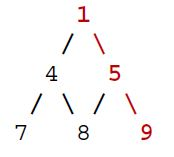
\includegraphics{Graficos/tree}
\end{center}

You need to walk in a tree on the path that has a maximum summation (e.g., 1 + 5 + 9 = 15). Numbers in each summation cannot cross into different links (e.g., 5+7 is illegal). Then, your intermediate task is to calculate 2 numbers for alphabet extraction. The first number is calculated from $\sum_{i=1}^{n}{i^2}$ where i is a number along the maximum summation path and n is the height of a tree. The second number is a summation of the maximum path $\sum_{i=1}^{n}{i}$. Regarding to the example above, the first number = 1 + 25 + 81 = 107 and the second number = 1 + 5 + 9 = 15. \\

Finally, these two numbers are transformed into two lower case alphabets from ``a'' to ``z'' respectively, where ``a'' is used for 0 and ``z'' is used for 25. Since there are only 26 alphabets, a number greater than 25 will reuse the same set of alphabets. For example, 107 = ``d'' and 15 = ``p'' (that is, the first alphabet ``a'' = 0, or 26, or 52 etc). \\

Write a program to find the 2 mysterious alphabets from a given tree.

\InputFile

The first line of input contains the height ($n$) of a tree ($0 \le n \le 100$). The second line contains unsigned integer numbers ($i$) in each level of a tree ($0 \le i \le 100$), consecutively. Assume that there is only one maximum path in a tree. \\


\OutputFile

The first line contains two integer calculated from the rules above, and the second line contains 2 decoded alphabets.  \\


\Example

\input ejemplos/tree.txt


URL:\\ 
http://coj.uci.cu/24h/problem.xhtml?pid=2632

\end{problema}
